\documentclass{beamer}
\usepackage[utf8]{inputenc}
\usepackage{graphicx}

\hypersetup{
    colorlinks,%
    citecolor=blue,%
    filecolor=blue,%
    linkcolor=blue,%
    urlcolor=blue 
    %urlcolor=mygreylink     % can put red here to better visualize the links
}

\author[Sowmya Vajjala]{Instructor: Sowmya Vajjala}

\title[LING 520]{LING 520: Computational Analysis of English}
\subtitle{Semester: FALL '16}

\date{13 October 2016}

\institute{Iowa State University, USA}
%%%%%%%%%%%%%%%%%%%%%%%%%%%

\begin{document}

\begin{frame}\titlepage
\end{frame}

\begin{frame}
\frametitle{Class Outline}
\begin{itemize}
\item Text Classification: Review of tuesday
\item Naive Bayes classifier
\item K-Nearest neighbour classifier
\item Text classification and NLTK
\end{itemize}
\end{frame}

\begin{frame}
\frametitle{What is text classification?}
\begin{itemize}
\item Assuming we have some example texts which have some pre-defined class/category labels,
\item text classification has this goal: developing a "model" of categorization based these example texts (training data)
\item ... and using this model to assign categories to new texts.
\end{itemize}
\end{frame}

\begin{frame}
\frametitle{Text Classification - Process}
\begin{itemize}
\item Step 1: You have some collection of texts labeled with some categories, which you will use as training data for your model \pause
\item Step 2: You design some features that you think can distinguish between these categories (kitchen sink strategy or hand-crafted) \pause
\item Step 3: Convert those texts into feature vectors. \pause
\item Step 4: Develop or use an existing learning algorithm that can learn a classification function based on the values of all these features for the texts \pause
\item Step 5: Evaluate the classification based on some measure. Tune your classifier with better features, better learning algorithm or with more data (or all of those) \pause
\item Step 6: Stop when you are satisfied, and deploy your classifier in some real world application \pause \\ (and discover all that research still does not result in material benefit!)
\end{itemize}
\end{frame}

\begin{frame}
\frametitle{Measuring Success in Learning}
Multiple ways. Depends on the nature of your dataset, and your application.
\begin{itemize}
\item Prediction accuracy on test set: typically used in most ML evaluation for text, images, videos, all sorts of things
\item False positive rate (Type 1 Error), False negatives (Type 2 error) - typically in medical applications
\item Precision (TP/(TP+FP)), Recall (TP/(TP+FN)), F-score (2PR/(P+R)) - typically in information retrieval, text classification
\item Revenue increase - in e-commerce applications
\end{itemize}
\end{frame}

\begin{frame}
\frametitle{Some commonly used features in text classification}
\begin{itemize}
\item ngrams (word, character, POS, mixed representations)
\item specific hand-crafted features: e.g., number of spelling errors, number of dependent clauses per clause, number of preposition phrases per sentence etc.
\item feature representation: binary (presence or absence), count (number of occurrences), ratios etc.
\end{itemize}
\end{frame}

\begin{frame}
\frametitle{Some commonly used learning algorithms}
\begin{itemize}
\item Naive bayes classifier
\item K-nearest neighbors classifier
\item Logistic regression
\item Decision trees
\item Random forests
\item Support vector machines
\item neural network classifiers
\end{itemize}
.. etc. \\ Note: I will only give an overview of how these work. Details are found in machine learning classes.
\end{frame}

\begin{frame}
\frametitle{}
\Large Naive Bayes classifier
\end{frame}

\begin{frame}
\frametitle{Naive Bayes Classifier}
\begin{itemize}
\item Let us say I have a collection of emails (E1, E2 ... En). My problem is to classify them as spam or non-spam.
\item Let us assume I already have some training data of 1000 emails labeled as Spam, 1000 labeled non-spam.
\item Bayes classifier solves the text classification problem using bayes rule. For some email E1\\
P(spam$|$E1) = P(spam)*P(E1$|$spam)/P(E1) \\
P(non-spam$|$E1) = P(non-spam)*P(E1$|$non-spam)/P(E1) 
\item if first probability is higher than second, the email is spam. Else, it is non-spam.
\item Since this is a comparison, we can ignore the denominator.
\end{itemize}
\end{frame}

\begin{frame}
\frametitle{Naive Bayes - continued}
Let us take individual terms:
\begin{itemize}
\item P(spam), P(non-spam): prior probability of seeing a spam or non-spam message. If your training data has 400 spam and 100 non-spam messages, what are P(spam) and P(non-spam)? \pause
\item P(E1$|$spam),P(E1$|$non-spam): likelihood that the email is actually spam or non-spam based on our training data. How do we get this?
\item If we take a "bag of words" approach, and consider each word as a feature, each unique word in the email becomes a feature. 
\item If an email has only two words: "my mail", P(E1$|$spam) = P(my$|$spam)*P(mail$|$spam). P(E1$|$non-spam) = P(my$|$non-spam)*P(mail$|$non-spam). \pause
\item If an email has 100 words, P(E1$|$spam) and P(E1$|$non-spam) are products of 100 conditional probabilities. You assign E1 to spam if P(E1$|$spam) is higher than P(E1$|$non-spam) and vice-versa.
\end{itemize}
\end{frame}

\begin{frame}
\frametitle{Naive Bayes - conclusion}
\begin{itemize}
\item Assumption: Each feature is independent of the other.
\item There is no in-built way to account for inter-correlation between features
\item So, this assumption does not really tell the whole story about what is happening. But it works for predictive modeling! 
\end{itemize}
\end{frame}

\begin{frame}
\frametitle{}
\Large K-nearest  neighbors classifier
\end{frame}

\begin{frame}
\frametitle{k-NN classifier}
\begin{itemize}
\item Idea: A document belongs to the majority category among its k-neighbors. \pause
\item Let us say my classification problem is: classifying movie reviews into three groups - positive, negative, neutral.
\item My training data: say 500 examples for each of these categories.
\item Let us say I am using only two features: Use of positive adjectives, Use of negative adjectives 
\item If I say my k is 5, when I have to classify a new review, and 3 of its neighbors on this feature space have category "positive", 1 has "negative", 1 has "neutral", I will choose "positive" as the category for this new review, because majority of my k neighbors  have "positive".
\item What is neighborhood? - any measure of distance. 
\end{itemize}
\end{frame}

\begin{frame}
\frametitle{k-NN classifier - 2D example}
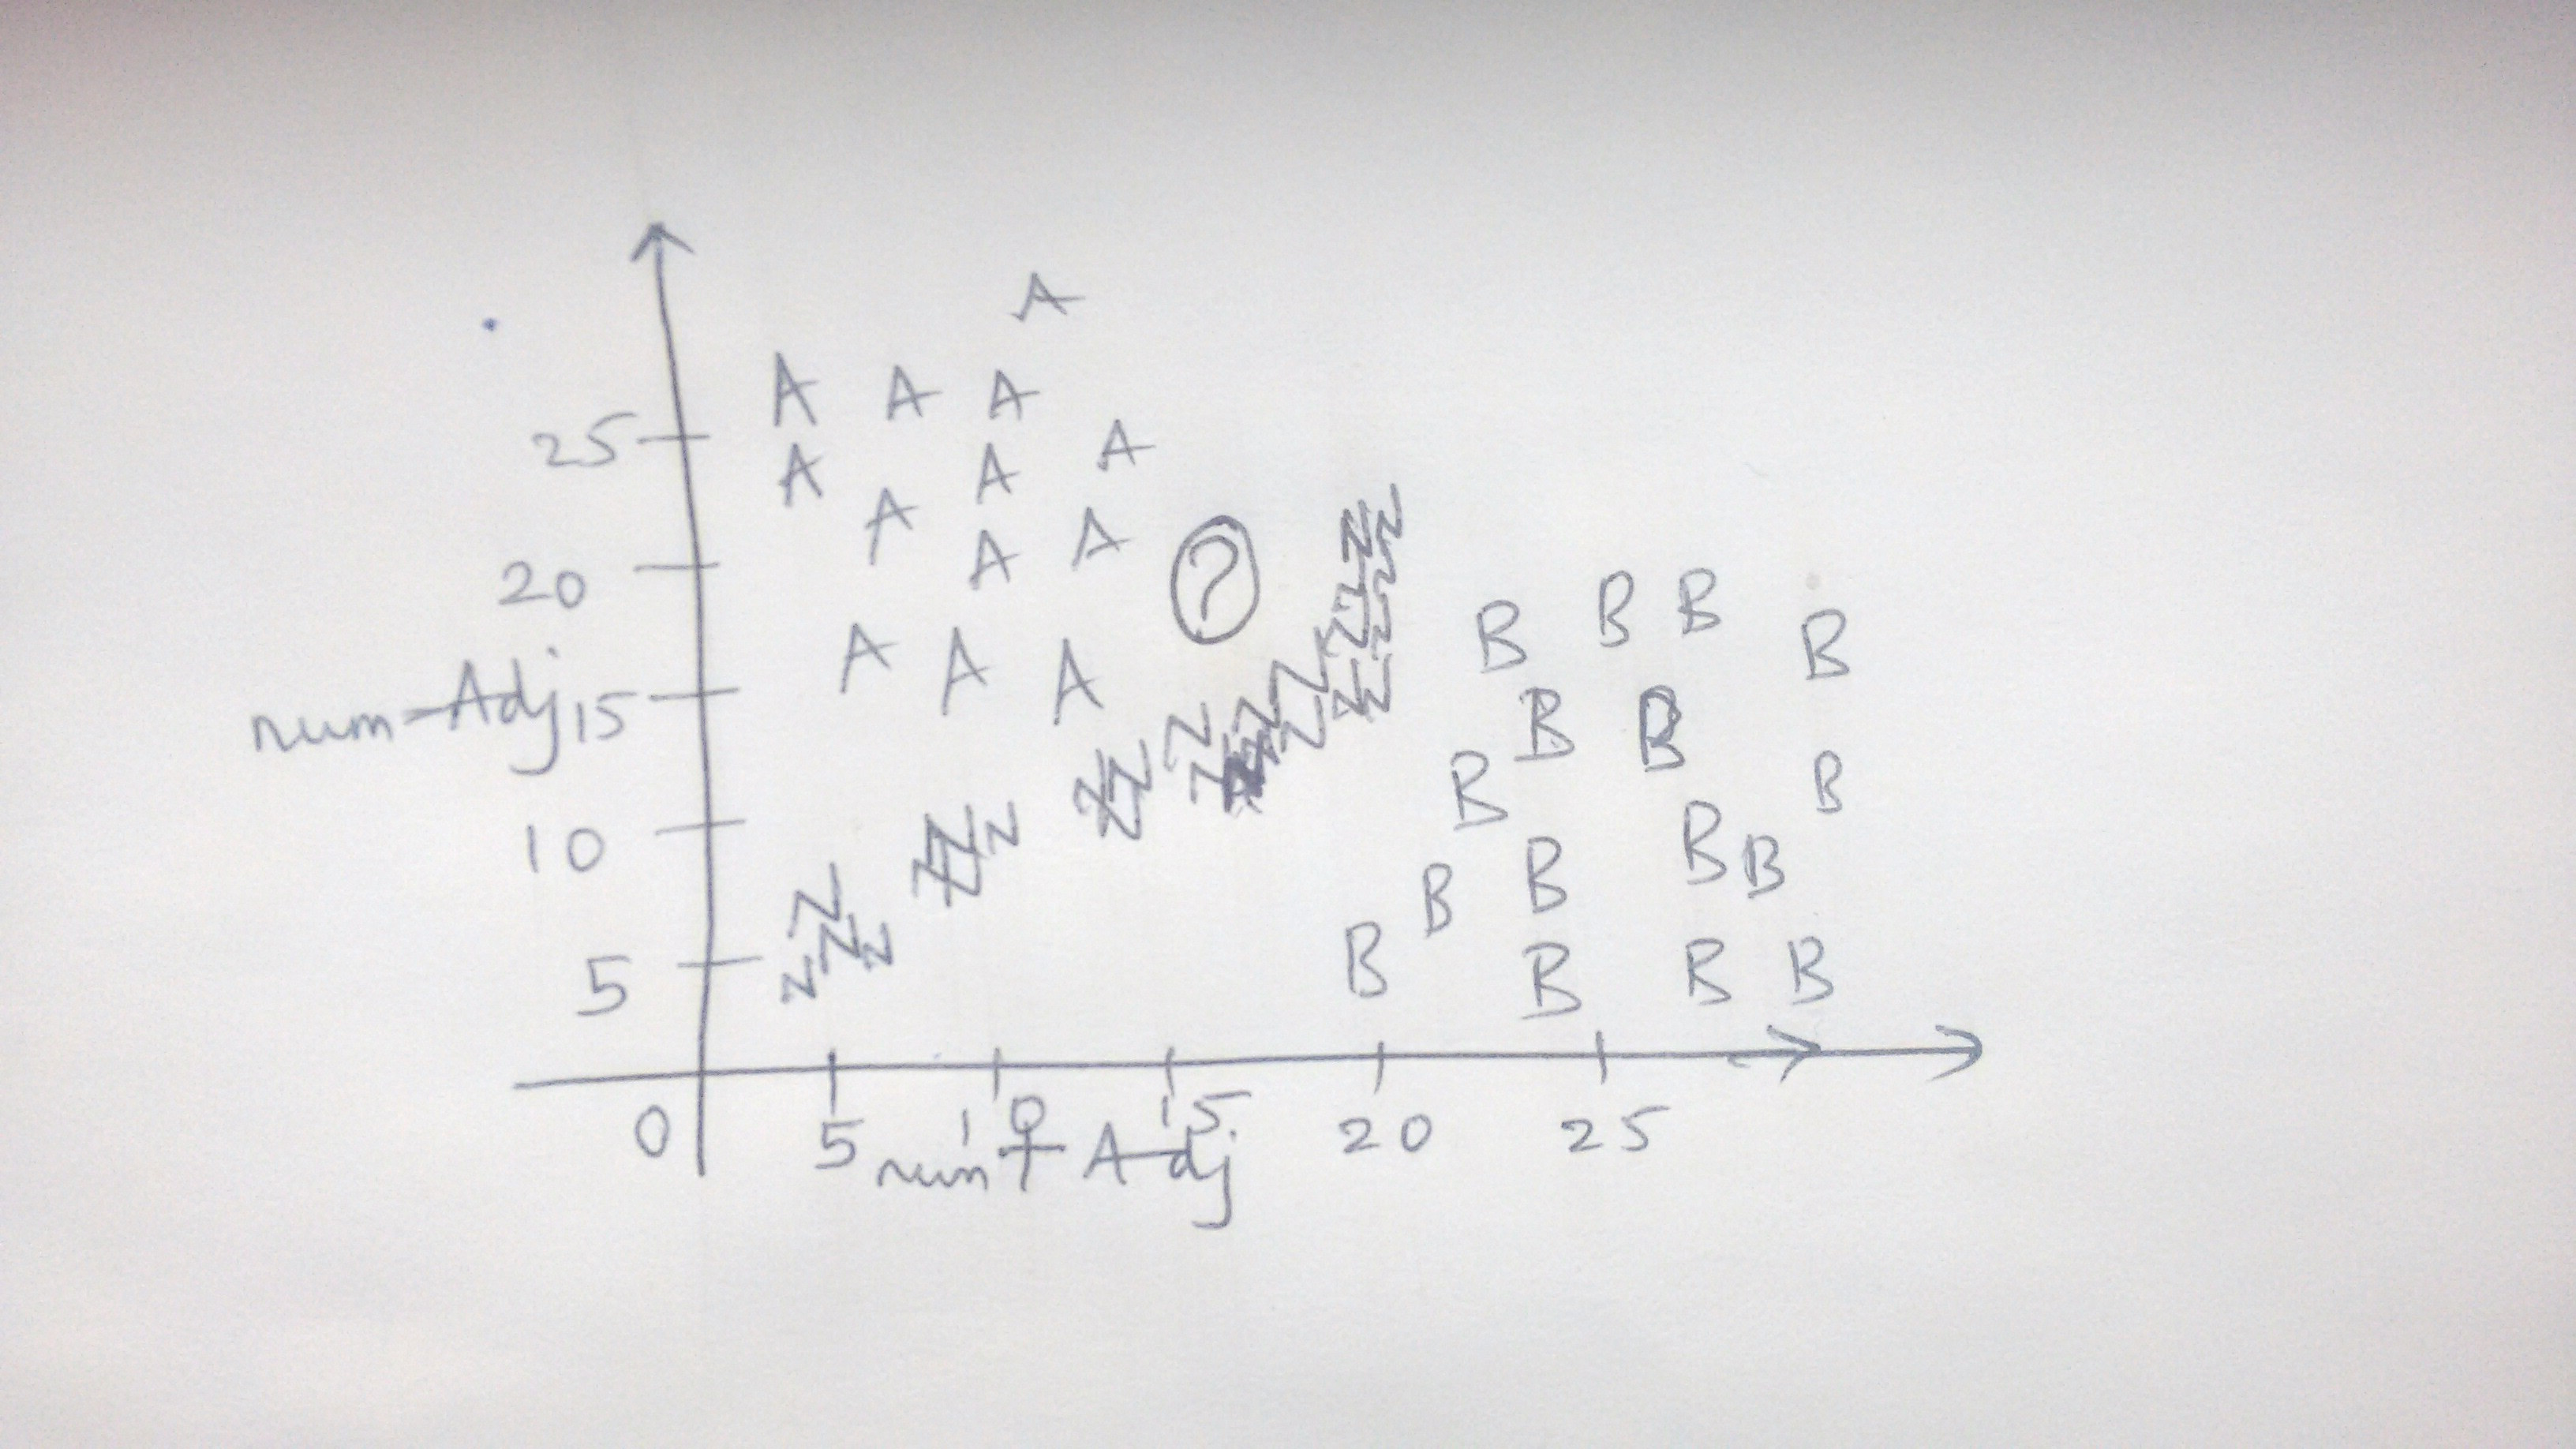
\includegraphics[width=0.9\textwidth]{KNN-Example.jpg}
\end{frame}

\begin{frame}
\frametitle{kNN - conclusion}
\begin{itemize}
\item Also called "instance based classifier" or "lazy learner"
\item Does not really have a "model" or "function". All computation of near-ness or far-ness happens during actual classification
\item If you have large amounts of training data, and large feature set, this will become extremely slow. 
\item selecting k is heuristic.
\item relationship between features is till not considered. Features are considered independent of each other.
\end{itemize}
\end{frame}


\begin{frame}
\frametitle{NLTK and Text Classification}
\begin{itemize}
\item Follow 1.1 and 1.2 in Chapter 6 and try to understand:
\begin{enumerate}
\item How to develop a classifier in Python using Naive Bayes algorithm
\item What exactly are the features in the example there?
\item What are the most informative features, and are they consistent between your and your neighbor's computer?
\item What is the classification accuracy? 
\item Let us say you want to add one more feature - starting letter. How do you do that?
\end{enumerate}
\end{itemize}
\end{frame}

\begin{frame}
\frametitle{Next Week}
\begin{itemize}
\item Brief overview of some more classification algorithms: Logistic Regression, Random Forests, Support Vector Machines
\item LightSide text mining toolkit, and Assignment 4 Description
\item Conclusion of text classification
\item Recap of concepts so far + Tutorial on Friday evening (21st October)
\item Submit Assignment 3 on time!
\end{itemize}
\end{frame}

\end{document}



